\documentclass[runningheads,a4paper,draft]{llncs} % TODO remove draft mode
\usepackage{booktabs}
\usepackage[hidelinks]{hyperref}
\usepackage{pgfplots}
\usepgfplotslibrary{fillbetween}
\usetikzlibrary{patterns}
\usepackage{multicol} % For 2 columned bullet point list
\usepackage{caption} % To improve laf of captions (also imported by subcaption)
\usepackage{mathtools} %For = aligned equations
\usepackage[final]{listings} %For microbenchmark code listing TODO: final prevents draft mode hiding listings. Remove for publication.
\usepackage{subcaption} % For putting figures 2-up
\usepackage[T1]{fontenc} % For literal \{ and \} in author emails
\pgfplotsset{compat=1.12}
%Power Optimised Software Envelope



\author{Stephen Roberts\inst{1} \and Stephen Jarvis\inst{1} \\ 
Chris January\inst{2} \and Jonathan Byrd\inst{2}}

\institute{The University of Warwick \\
  \email{\{S.I.Roberts, S.A.Jarvis\}@warwick.ac.uk}
\and
  Allinea Software
}

\authorrunning{Stephen Roberts et al.}
\title{POSE: A New Technique to Guide Energy Aware Code Optimisation}

\newcommand{\DRAFT}[1]{•}
\renewcommand*{\sectionautorefname}{Section} % make sec: autorefs capitalized.

\date{}
%COMMANDS

\newcommand{\todo}[1]{•}

\ifdefined\DRAFT
	\usepackage{color} %Used for colored text (TODO)
	\renewcommand{\todo}[1]{{\color{red} TODO: {#1}}} % comment me out for prod  
\fi 

\definecolor{printred}{RGB}{215,25,28}
\definecolor{printorange}{RGB}{253,174,97}
\definecolor{printyellow}{RGB}{255,255,191}
\definecolor{printgreen}{RGB}{145,180,130}
\definecolor{printblue}{RGB}{43,131,186}
\definecolor{printlilac}{RGB}{178,171,210}



\begin{document}
  \maketitle
  \begin{abstract}
Performance engineers are beginning to explore software-level optimisation as a means to reduce the energy consumed when running their codes.
This paper presents POSE, a mathematical and visual modelling tool which highlights the relationship between runtime and power consumption.
POSE allows developers to assess whether power optimisation is worth pursuing for their codes.

We demonstrate POSE by studying the power optimisation characteristics of codes from the Mantevo and Rodinia benchmark suites.
We show that LavaMD has the most scope for CPU power optimisation, with improvements in Energy Delay Squared Product ($ED^2P$) of up to 30.59\% feasible.
Conversely, MiniMD offers the least scope, with improvements to the same metric limited to 7.60\%.
We also show no power optimised version of MiniMD operating below 2.3 GHz can match the $ED^2P$ performance of the original code running at 3.2 GHz.
For LavaMD this limit is slightly less restrictive at 2.2 GHz.
\end{abstract}

  \section{Introduction}
Driven by Moore's Law, advances in processor design have delivered improvements in CPU performance for decades. As physical limits are reached, however, refinements to the same basic technologies are beginning to show diminishing returns. One side-effect of this is an unsustainable rise in system power use, which the US Department of Energy has identified as a primary constraint for exascale systems \cite{shalf:2011aa}.

Hardware manufacturers are increasingly prioritising energy efficiency in their processor designs~\cite{kurd:2014aa}.
In turn, some groups expect that software modifications will be required to fully exploit energy efficiency improvements in modern processors~\cite{shao:2013aa}.
They suggest this process will be analogous to the current practice of tuning code to reduce runtime.

This paper presents the Power Optimized Software Envelope (POSE) model.
POSE is a visual heuristic which provides performance engineers with insights into the optimization characteristics of their codes.
We demonstrate the utility of our model with a study of the runtime and CPU power usage characteristics of several popular benchmarks.

  \section{Approaches to Modelling}
\label{sec:approaches}
Performance modelling techniques enable the rapid exploration of large hardware and software design spaces.
In this section we describe various approaches to performance modelling and show where POSE fits into the picture.
\autoref{tab:approaches} divides the performance modelling ecosystem into categories based on model domain and granularity and provides examples for each.

\begin{table}
  \centering
  \caption{Performance Model Classifications}
  \setlength{\tabcolsep}{10pt}
  \begin{tabular}{lll}
  \toprule
    & \multicolumn{2}{l}{Domain}\\ \cmidrule(){2-3}
  Model Type  & Runtime & Energy \\
    \midrule
  Simulation & SST~\cite{rodrigues:2011aa} & McPAT~\cite{li:2009aa}  \\
  Analytical & Bunt~\cite{bunt:2013aa} & Karkhanis~\cite{karkhanis:2007aa} \\
  Heuristic & Roofline~\cite{williams:2009aa} & \textbf{This Work} \\
  \bottomrule
  \end{tabular}
  \label{tab:approaches}
\end{table}

\subsubsection{Simulators:} 
Tools like SST~\cite{rodrigues:2011aa} and McPAT~\cite{li:2009aa} gather data whilst executing a simplified representation of the original code.
These approaches can be extremely insightful, however constructing and validating representative simulations is often challenging.
They also tend to be expensive to run, sometimes even more so than the original code.

\subsubsection{Analytical Models:} This approach distils the structure and performance of a program into parameterised expressions.
Examples of this technique are found in the work of Bunt~et~al.~\cite{bunt:2013aa} and Karkhanis~et~al.~\cite{karkhanis:2007aa}.
These models run much faster than simulations, making them particularly useful when performing parameter sweeps.
Ensuring the model is expressive enough to capture all possible program behaviours is the biggest obstacle to this approach as it requires a deep understanding of the target application.

\subsubsection{Heuristic Models:}
This is the most abstract category of performance models and the one in which our work belongs.
Rather than attempting to faithfully represent an entire system, heuristic models provide a simplified analogy which helps developers to reason about particular properties of a code.

A popular example of this class is the Roofline~\cite{williams:2009aa} model.
Roofline frames the performance of an application in terms of its operational intensity and two system bottlenecks; off-chip memory bandwidth and floating point performance.
This simplification limits Roofline's use as a predictive model but it also means a developer can easily isolate the limiting factor of code performance and target their optimisation efforts accordingly.

The POSE heuristic serves as a preliminary `first cut' modelling technique intended to guide energy-aware optimisation efforts.
Our model provides an asymptotic analysis of the scope for optimisation in the power and runtime domains, allowing performance engineers to focus their efforts where they will be most beneficial.
POSE also takes after the Roofline model in that its insights can be presented in the form of a two-dimensional graphical representation.

  \section{Energy Aware Optimisation}
\label{sec:optimisation}

Energy is the integral of power consumed over time, or simply $E = \bar{P}t$.
As such, reducing the energy consumed by a code can be achieved either through shortening its runtime ($t$) with conventional optimisations or reducing the average power consumption ($\bar{P}$) with power optimisations.
The POSE heuristic enables performance engineers to compare the potential benefits of each approach and focus their efforts on whichever offers the greatest rewards.

Energy cost is a reasonable metric in cases where energy consumption is of paramount importance.
That said, relying on this metric leaves open the possibility of significant loss of runtime performance, limiting its usefulness in time-sensitive domains.
Metrics combining both runtime and energy costs have been developed to address this issue. 
The simplest of these is the Energy-Delay Product (EDP) metric \cite{gonzales:1995aa}, which is defined as follows:
\begin{align}
  EDP &= Energy \times Runtime \nonumber \\
      &= E \times t \nonumber \\
      &= \bar{P} \times t^2
  \label{eq:edp}
\end{align}

Several extensions to EDP have been proposed which assign different weights to each components in order to better reflect the demands of specific domains.
Common examples include Energy Delay Squared Product ($Et^{2}$) and Energy Delay Cubed Product ($Et^{3}$).
We refer to this as the $E^mt^n$ family of metrics, which also includes power ($E^1t^{-1}$), energy ($E^1t^0$) and time ($E^0t^1$) as members.

POSE is a general purpose heuristic which applies to all members of the $E^mt^n$ group with $m > 0$ and $n \geq 0$, and indeed any metric which increases in line with runtime and energy consumption.
That said, most of the examples within this paper use $Et^2$ as this has been shown to be the most suitable of the $E^mt^n$ metrics when considering a fixed micro-architecture \cite{brooks:2000aa}.

  \section{Power Optimised Software Envelope}
\label{sec:pose}

The POSE heuristic partitions the Energy/Runtime plane into areas with differing performance characteristics relative to some initial unoptimised code.
This section introduces the bounds which make up POSE and provides their derivations for the $E^mt^n$ family of metrics.
The only prerequisites of our model are that time and energy consumption can be accurately measured for the target platform.

\begin{figure}
\centering
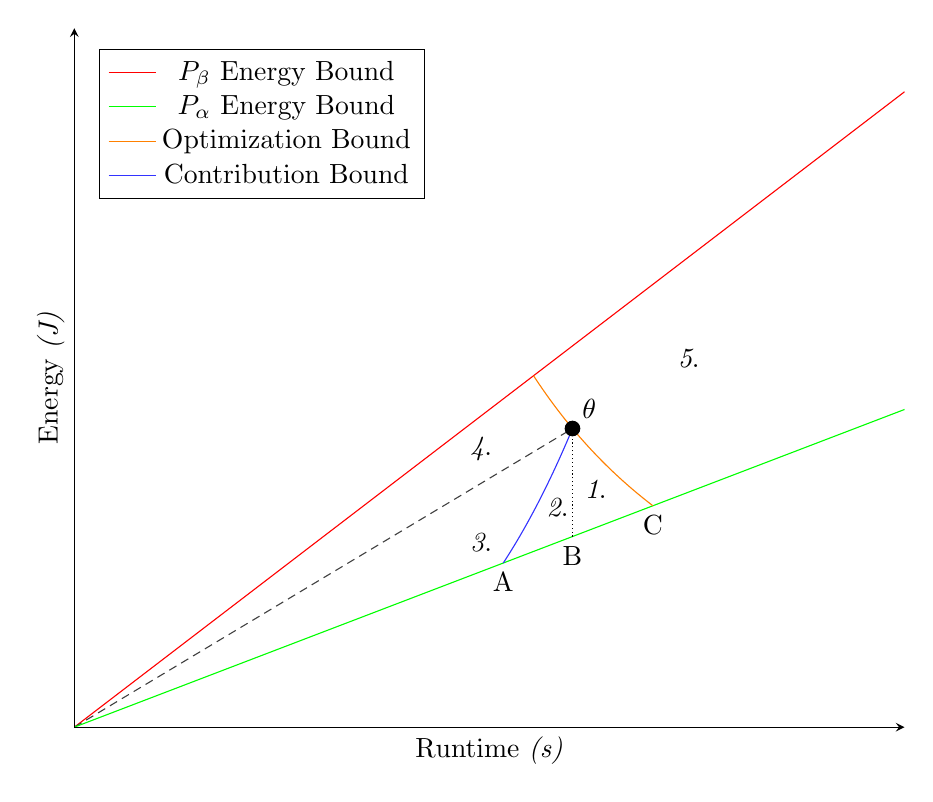
\begin{tikzpicture}
  \begin{axis}[ticks = none, 
    axis on top,
    axis x line=bottom,
    axis y line=left,
  	xlabel={Runtime \emph{(s)}},
    ylabel={Energy \emph{(J)}},    
    xmin=0, xmax=50,
    ymin=0, ymax=3300,
    width=\linewidth,
    legend style={legend pos=north west}
    ]

    %% Model Parameters %%
    \pgfmathsetmacro{\baselinepower}{30} % NOP code
    \pgfmathsetmacro{\rooflinepower}{60}
    \pgfmathsetmacro{\codepower}{47} 
    \pgfmathsetmacro{\codetime}{30}
    % Sadly, pgfplots sucks too much to calculate cube roots
    % These values are calculated with a ruby script in tools
    \pgfmathsetmacro{\anodex}{25.83028}
    \pgfmathsetmacro{\cnodex}{34.84283}
    \pgfmathsetmacro{\tnodex}{27.65477}

    \pgfmathsetmacro{\cnodey}{\cnodex * \baselinepower}
    \pgfmathsetmacro{\anodey}{\anodex * \baselinepower}
 
    %% Intermezzo Values %%
    \pgfmathsetmacro{\codeenergy}{\codepower * \codetime}
    \pgfmathsetmacro{\baselineenergy}{\baselinepower * \codetime}
    \pgfmathsetmacro{\rooflineenergy}{\rooflinepower * \codetime}
    \pgfmathsetmacro{\lowdisplayline}{(2 * \baselinepower + \codepower) / 3}
    \pgfmathsetmacro{\highdisplayline}{(1 * \rooflinepower + 1 * \codepower) / 2}

    % arguments: code power, code time, x - todo, apparently not supposed to do pgfmathparse
    \pgfmathdeclarefunction{metricbound}{3}{%
      \pgfmathparse{((#1 * #2^3) / #3^2)}%
    }
    \pgfmathdeclarefunction{definitionbound}{3}{%
      \pgfmathparse{((#1 / #2^3) * #3^4)}%
    }

    % BETA ROOFLINE BOUND
    \addplot[color=red, domain=\pgfkeysvalueof{/pgfplots/xmin}:\pgfkeysvalueof{/pgfplots/xmax}] {\rooflinepower * x};
    \addlegendentry{$P_{\beta}$ Energy Bound}

    %const power diagonal
    \addplot[color=darkgray, densely dashed, forget plot, %forget plot prevents legend entry
            domain=\pgfkeysvalueof{/pgfplots/xmin}:\codetime] {\codepower * x}; 

    % ALPHA BASELINE BOUND 
    \addplot[color=green, domain=\pgfkeysvalueof{/pgfplots/xmin}:\pgfkeysvalueof{/pgfplots/xmax}] {\baselinepower * x};
    \addlegendentry{$P_{\alpha}$ Energy Bound} 

    \addplot[color=orange, domain=\tnodex:\cnodex] { metricbound(\codepower, \codetime, x)};
    \addlegendentry{Optimization Bound}

    \addplot[color=blue!80, domain=\anodex:\codetime] { definitionbound(\codepower, \codetime, x)};
    \addlegendentry{Contribution Bound}

    % Constant Time, Energy Dashes
    %vertical
    \draw[densely dotted] ({axis cs:\codetime,\baselineenergy}) -- ({axis cs:\codetime,\codeenergy});

    \node[circle,fill,inner sep=2pt] at (axis cs:\codetime,\codeenergy) {};
    \node[above right] at (axis cs:\codetime,\codeenergy) {$\theta$};
    \pgfmathsetmacro{\oneycoord}{\lowdisplayline * 31.4}
    \node at (axis cs:31.4,\oneycoord) {\textit1.};
    \pgfmathsetmacro{\twoycoord}{\lowdisplayline * 29.1}
    \node at (axis cs:29.1,\twoycoord) {\textit2.};
    \pgfmathsetmacro{\threeycoord}{\lowdisplayline * 24.5}
    \node at (axis cs:24.5,\threeycoord) {\textit3.};
    \pgfmathsetmacro{\fourycoord}{\highdisplayline * 24.5}
    \node at (axis cs:24.5,\fourycoord) {\textit4.};
    \pgfmathsetmacro{\fiveycoord}{\codepower * 37}
    \node at (axis cs:37,\fiveycoord) {\textit5.};
    
    \node [below] at ({axis cs:\anodex, \anodey}) {A};
    \node [below] at ({axis cs:\codetime,\baselineenergy}) {B};
    \node [below] at ({axis cs:\cnodex, \cnodey}) {C};
    %\node [below, name intersections={of=metric bound and baseline}] at (intersection-1) {C};


 \end{axis}
\end{tikzpicture}

\caption{$E^1t^2$ Power Optimised Software Envelope}
\label{fig:technique}
\end{figure}

\subsection{Feasible Performance Envelope}
POSE is built around the concept of a \emph{Feasible Performance Envelope}.
We construct this by plotting lines of gradient $P_{max}$ and $P_{min}$ in \autoref{fig:technique}.
These values represent the maximum and minimum rates of power consumption which can occur during normal operation of the target platform.
The $\langle Runtime, Energy\rangle$ costs incurred by running any given code $\theta$ under similar conditions must be represented somewhere within this envelope.

\subsection{Optimisation Bound}
To constrain our search space further we consider the metric we wish to reduce.

\begin{definition}
For logically equivalent codes $\theta$ and $\lambda$, the transformation ${\theta \to \lambda}$ is a valid optimisation with respect to cost metric $M$ if and only if ${M(\lambda) < M(\theta)}$.
\label{def:optimisation}
\end{definition}

We plot a curve passing through $\theta$ linking all points where ${M(\lambda) = M(\theta)}$. By \autoref{def:optimisation} any optimised versions of $\theta$ must exist below this bound.
Naturally the equation for the Optimisation Bound depends on the metric we are optimising for.
\autoref{fig:technique} shows the Optimisation Bound for $E^1t^2$.
The general form of this bound for the $E^mt^n$ family of metrics is derived as follows:
\begin{align}
 {E_\lambda}^m{t_\lambda}^n &= {E_\theta}^m{t_\theta}^n \nonumber \\
 {E_\lambda}^m &= \frac{{E_\theta}^m{t_\theta}^n}{{t_\lambda}^n} \nonumber \\
  E_\lambda &= (\frac{{E_\theta}^m{t_\theta}^n}{{t_\lambda}^n})^\frac{1}{m}
\label{eq:optimisation}
\end{align}

\subsection{Contribution Bound}
Our second bound considers what it means to optimise for reduced power draw.

\begin{definition}
An optimisation $\theta \to \lambda$ with respect to metric $M$ is a power optimisation if the reduction in power draw it delivers is responsible for the majority of the improvement in $M$.
\label{def:poweropt}
\end{definition}

We plot a curve through $\theta$ linking all points for which power and runtime factors contribute to $M$ in the same ratio as our original code.
By \autoref{def:poweropt} any power-optimised versions of $\theta$ must lie below this Contribution Bound.
Again the equation for the Contribution Bound depends on the metric chosen. 
\autoref{fig:technique} shows the bound for $E^1t^2$ while the general form for $E^mt^n$ metrics is derived as follows:
\begin{align}
\frac{{P_{\lambda}}^m}{{t_{\lambda}}^{m+n}} &= \frac{{P_{\theta}}^m}{{t_{\theta}}^{m+n}} \nonumber \\
 {P_{\lambda}}^m &= \frac{{P_{\theta}}^m}{{t_{\theta}}^{m+n}} \times {t_\lambda}^{m+n} \nonumber \\ 
 {E_{\lambda}}^m &= \frac{{P_{\theta}}^m}{{t_{\theta}}^{m+n}} \times {t_\lambda}^{m+n+1} \nonumber \\ 
  E_{\lambda} &= (\frac{{P_{\theta}}^m}{{t_{\theta}}^{m+n}} \times {t_\lambda}^{m+n+1})^{\frac{1}{m}} 
\end{align}

It makes sense to use the most appropriate tools while searching for optimisations.
If an optimisation yields dramatic reductions in runtime with only minor reductions in power consumption then it is reasonable to classify it as a runtime optimisation and state that conventional time-based profilers and performance engineering tools are better suited to finding it.
It is the Contribution Bound which enables our model to make this distinction.
\subsection{Optimisation Limit}
The bounds described thus far delineate those areas of the Energy/Runtime plane in which runtime and power optimised versions of a given code may exist.
The final component of POSE is the Optimisation Limit.
This partitions runtime optimisations into those which strictly dominate all power optimisations and those which could potentially be outperformed by them.

This limit is related to the Optimisation Bound and is likewise based on \autoref{eq:optimisation}.
It connects all points with the same value for $M$ as the maximally power-optimised point in our envelope.
All optimisations below this limit strictly dominate any possible power optimisation.

\section{POSE Insights}
\label{sec:insights}
The POSE Model partitions the feasible performance envelope from \autoref{fig:technique} into several areas.
Potential optimisations can be classified according to which of the following labelled areas they appear in:
\begin{multicols}{2}
\begin{enumerate}
\item Strong Runtime Optimisation
\item Weak Runtime Optimisation
\item Power Optimisation
\item Performance Degradation  
\end{enumerate}
\end{multicols}
Area \textbf{1} encompasses all points with a better $M$ value than the best case power optimisation for $\theta$.
Area \textbf{2} encompasses all possible runtime optimisations which have a better performance than $\theta$ in terms of $M$ yet may in turn be beaten by some power optimised version of $\theta$.
Area \textbf{3} contains all optimised versions of $\theta$ for which reductions in $M$ are due primarily or entirely to reductions in power consumption.
Finally, area \textbf{4} corresponds to all codes with strictly worse performance than $\theta$.

A key strength of POSE is that it produces quantitative and actionable insights relating directly to properties of the code.
These insights fall into one of two broad categories, which taken together allow a performance engineer to decide if power optimisation is likely to prove worthwhile.

The first of these categories relates to how much benefit may be offered by power optimisation.
Taking the difference in energy between point $\theta$ and $D$ gives us an upper limit on the amount of energy which can be saved by power optimisation. 
Similarly, the value $M(\theta) - M(C)$ bounds the amount of improvement in our metric we can expect to see from power optimisation.

The second category indicates how much scope a code has for power optimisation.
The difference in runtime between intersect $E$ and $\theta$ represents the maximum increase in runtime we could feasibly trade off to achieve a slower yet more energy efficient code.
The value $t_\theta / t_B$ represents the smallest speed-up which would guarantee a code which outperformed $\theta$ with respect to $M$.
Finally, $t_\theta / t_A$ is the smallest speed-up guaranteed to outperform any power optimised version of $\theta$.
\begin{figure}
\centering
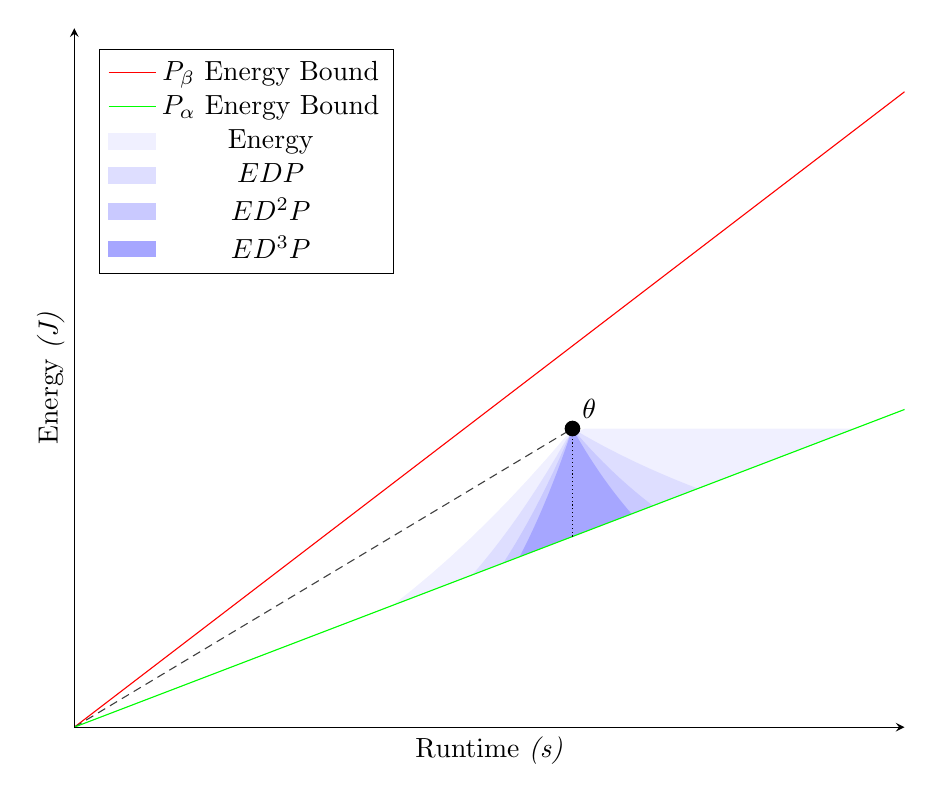
\begin{tikzpicture}
  \begin{axis}[ticks = none, 
    axis on top,
    axis x line=bottom,
    axis y line=left,
  	xlabel={Runtime \emph{(s)}},
    ylabel={Energy \emph{(J)}},    
    xmin=0, xmax=50,
    ymin=0, ymax=3300,
    width=\linewidth,
    legend style={legend pos=north west}
    ]

    %% Model Parameters %%
    \pgfmathsetmacro{\baselinepower}{30} % NOP code
    \pgfmathsetmacro{\rooflinepower}{60}
    \pgfmathsetmacro{\codepower}{47} 
    \pgfmathsetmacro{\codetime}{30}




    %% Intermezzo Values %%
    \pgfmathsetmacro{\codeenergy}{\codepower * \codetime}
    \pgfmathsetmacro{\baselineenergy}{\baselinepower * \codetime}
    \pgfmathsetmacro{\rooflineenergy}{\rooflinepower * \codetime}
    \pgfmathsetmacro{\lowdisplayline}{(2 * \baselinepower + \codepower) / 3}
    \pgfmathsetmacro{\highdisplayline}{(1 * \rooflinepower + 1 * \codepower) / 2}

    % arguments: code power, code time, x, n 
    \pgfmathdeclarefunction{metricbound}{4}{%
      \pgfmathparse{((#1 * #2^(#4 + 1)) / #3^#4)}%
    }
    \pgfmathdeclarefunction{definitionbound}{4}{%
      \pgfmathparse{((#1 / #2^(#4 + 1)) * #3^(#4 + 2))}%
    }
 
    % BETA ROOFLINE BOUND
    \addplot[color=red, domain=\pgfkeysvalueof{/pgfplots/xmin}:\pgfkeysvalueof{/pgfplots/xmax}] {\rooflinepower * x};
    \addlegendentry{$P_{\beta}$ Energy Bound}

    %const power diagonal
    \addplot[color=darkgray, densely dashed, name path=constpwr, forget plot, %forget plot prevents legend entry
            domain=\pgfkeysvalueof{/pgfplots/xmin}:\codetime] {\codepower * x}; 

    % ALPHA BASELINE BOUND 
    \addplot[color=green, name path=basebound, domain=\pgfkeysvalueof{/pgfplots/xmin}:\pgfkeysvalueof{/pgfplots/xmax}] {\baselinepower * x};
    \addlegendentry{$P_{\alpha}$ Energy Bound} 

    % Constant Time vertical dots
    %vertical
    \draw[densely dotted] ({axis cs:\codetime,\baselineenergy}) -- ({axis cs:\codetime,\codeenergy});

    % Sadly, pgfplots sucks too much to calculate cube roots
    % Domain values are calculated with a ruby script in tools

    %% Energy Area %%
    \addplot[name path=energy, draw=none, domain=19.14894:47, forget plot]{ min(definitionbound(\codepower, \codetime, x, 0),metricbound(\codepower, \codetime, x, 0))};
    \addplot[blue!6] fill between[of=energy and basebound];
    \addlegendentry{Energy}

    %% Energy Delay Product Area %% 
    \addplot[name path=edp, draw=none, domain=23.96806:37.54997, forget plot] { min(definitionbound(\codepower, \codetime, x, 1),metricbound(\codepower, \codetime, x, 1))};
    \addplot[blue!13] fill between[of=edp and basebound];
    \addlegendentry{$EDP$}

    %% Energy Delay Squared Product Area ##
    \addplot[name path=edtwop, draw=none, domain=25.83028:34.84283, forget plot] { min(definitionbound(\codepower, \codetime, x, 2),metricbound(\codepower, \codetime, x, 2))};
    \addplot[blue!21] fill between[of=edtwop and basebound];
    \addlegendentry{$ED^2P$}

    %% Energy Delay Cubed Product Area ##
    \addplot[name path=edthreep, draw=none, domain=26.81496:33.56336, forget plot] { min(definitionbound(\codepower, \codetime, x, 3),metricbound(\codepower, \codetime, x, 3))};
    \addplot[blue!35] fill between[of=edthreep and basebound];
    \addlegendentry{$ED^3P$}




     \node[circle,fill,inner sep=2pt] at (axis cs:\codetime,\codeenergy) {};
    \node[above right] at (axis cs:\codetime,\codeenergy) {$\theta$};
  \end{axis}
\end{tikzpicture}

\caption{POSE for Different Metrics}
\label{fig:multimetric-technique}
\end{figure}

It is worth restating that POSE is a metric-agnostic heuristic. \autoref{fig:multimetric-technique} shows how the POSE heuristic varies with choice of metric using Energy ($E^1t^0$) and Energy Delay Squared Product $E^1t^2$ as examples. POSE offers the same insights regardless of the metric chosen.


  \section{Investigation}
\label{sec:investigation}
\noindent
This section demonstrates POSE by investigating the scope for CPU power optimisation for a selection of codes from the Mantevo~\cite{heroux:2009aa} and Rodinia~\cite{che:2009aa} benchmark suites.

CPU energy consumption accounts for a significant portion of the energy used by high performance systems~\cite{rong:2010aa} and is therefore a prime target for optimisation.
It can also be measured accurately on commodity hardware~\cite{hackenberg:2013aa} making it a suitable candidate for POSE modelling.
Our experiments were carried out on an Intel Core i5-3470 Ivy Bridge CPU which supports Intel's Running Average Power Limit (RAPL) technology~\cite{david:2010aa}.

\subsection{CPU Power Consumption}
\label{ssec:cpupower}
\noindent
Current processors are based on Complimentary Metal Oxide Semiconductor (CMOS) technology.
\autoref{eq:totpwr} separates the power draw of CMOS chips into its component parts, of which dynamic and leakage power are the most significant.
\begin{equation}
\label{eq:totpwr}
P_{tot} = P_{dyn} + P_{leak} + P_{other}
\end{equation}
Dynamic power is consumed when logic gates change state.
Leakage power exists because at microscopic scales the insulating properties of silicon break down, allowing some current to escape even when gates remain inactive.
Other forms of power dissipation exist, however their effects are relatively minor \cite{kaxiras:2008aa}.
\begin{gather}
P_{dyn} \propto CV^{2}Af \label{eq:dynpwr} \\
P_{leak} = V\times I_{leak} \label{eq:staticpwr}
\end{gather}
\autoref{eq:dynpwr} is a common approximation for dynamic power in which $C$ denotes load capacitance, $V$ the supply voltage, $A$ the activity factor and $f$ the clock frequency.
\autoref{eq:staticpwr} is a simplified expression for leakage power which exploits the fact that leakage current ($I_{leak}$) is invariant to processor workload~\cite{kim:2003aa}.

Activity factor captures the fraction of logic elements which change state each clock cycle.
Frequency and supply voltage vary in tandem, taking values from a set of \textit{(frequency, voltage)} pairs known as P-states.
Dynamic Voltage and Frequency Scaling (DVFS) selects a P-state based on workload, or places the CPU into an energy saving mode if no work is available.
Finally, capacitance and leakage current are constants dictated by hardware design.

Processor architecture also plays a significant roll in determining total power consumption.
Each core in a multi-core architecture operates independently with its own activity factor and in some cases P-state.
As a result, \autoref{eq:totpwr} should be summed across all cores to arrive at a value for the entire processor.

\subsection{Feasible Performance Envelope}
\noindent
The first step in applying POSE is to construct a feasible performance envelope.
Many manufacturers publish power dissipation figures for their hardware, however for safety reasons these are usually conservative estimates.
POSE works best when the minimum and maximum power bounds are as tight as possible, therefore we determine $P_{\min}$ and $P_{\max}$ empirically.

We specify power benchmarks using $(S,A,C)$ tuples, with P-state $S$, activity factor $A$ and active core count $C$.
Our $P_{min}$ and $P_{max}$ benchmarks should reflect the range of values these properties can take for a given code $\theta$.
This notion is formalised by \autoref{eq:pbench}.
\begin{align}
  \label{eq:pbench}
  \begin{split}
    P_{min} &= (S_{min}, A_{min}, C_{min}~\vert~\theta) \\
    P_{max} &= (S_{max}, A_{max}, C_{max}~\vert~\theta) 
  \end{split}
\end{align}
The values of $S$, $A$, and $C$ depend on the code and the nature of the optimisations being considered.
POSE models for inherently serial codes should be constructed using single threaded benchmarks where $C_{min} = C_{max} = 1$, for example.

The \texttt{cpufrequtils} package allows us to override DVFS and manually set the desired P-state $S$.
We control the number of active cores $C$ by specifying the number of threads used by our benchmarking routines and pinning each one to its own core to prevent migration.
The remaining property is activity factor, which is influenced by benchmark code.

\begin{figure}[ht]
\centering
\lstset{basicstyle=\ttfamily\footnotesize\bfseries, frame=tb} %small bold text, lines top and bottom
\lstinputlisting[]{lst/alpha_benchmark.c}
\caption{Activity Factor $\alpha$ Benchmark Code}
\label{fig:microbench}
\end{figure}

We define the range of values that $A$ can take for some fixed $S$ and $C$ as $[\alpha,~\beta]$ where $0 < \alpha < \beta < 1$.
Our code for targeting activity factor $\alpha$ is given in \autoref{fig:microbench}.
This benchmark executes a single \texttt{jmp} instruction each clock cycle, preventing instruction pipelining.
It performs no floating point or integer calculations and no memory accesses while keeping control logic to a minimum.

Non-trivial codes perform more work per unit time than our minimal benchmark.
This additional work means more transistors changing state per cycle, and hence a higher activity factor.
The only exception occurs when applications are blocked for long periods, allowing the processor to enter an idle state.
This can be addressed by adding delays to the benchmark if necessary.

FIRESTARTER~\cite{hackenberg:2013ab} serves as our benchmark for activity factor $\beta$.
This tool is designed to trigger near-peak power consumption across a range of x86\_64 processors.
It consists of hand optimised assembly routines which raise the activity factor above the level achievable with high level languages.
Prime95 and Linpack were also evaluated as potential $\beta$ benchmarks however they were consistently outperformed by FIRESTARTER.

The benchmark parameter space is small enough to fully characterise a processor by measuring all $(S,A,C)$ configurations.
Benchmarking runs lasted for 120 seconds to allow enough time for power readings to stabilise.
We extended the Unix \texttt{time} binary to gather power consumption figures using RAPL.
Techniques described by Hahnel~et~al.~\cite{hahnel:2012aa} were used to promote measurement accuracy.
Results are presented in \autoref{tab:fpe_params}, which identifies P-states by their frequency component.

\begin{table}
  \scriptsize
  \centering
  \caption{Feasible Performance Envelope Parameters (W)}
  \label{tab:fpe_params}
  \input{tab/tex/fpe_params.tex}
\end{table}

\subsection{POSE Models for Code Optimisation}
\noindent
Having characterised our system we now proceed to build POSE models for benchmarks in the Mantevo and Rodinia suites.
These codes were compiled with ICC version 14.0.0.
Codes were run with default configurations where available.
The energy and runtime costs associated with each code is given in \autoref{tab:code_metrics}.

\begin{table}
  \scriptsize
  \centering
  \caption{Code Metrics for $S = 3.2\text{ GHz}$, $C = 4$}
  \label{tab:code_metrics}
  \input{tab/tex/code_metrics.tex}
\end{table}

All codes ran in parallel across four cores.
They also spent a negligible amount of time waiting for resources. 
This allowed the CPU to run at its maximum supported frequency of 3.2 GHz.
For the first stage of this investigation we disregard optimisations which reduce parallelism ($C < 4$) or processor throughput (S < 3.2 GHz).
The benchmark configurations used were $(\text{3.2 GHz}, \alpha, 4)$ for $P_{min}$ and $(\text{3.2 GHz}, \beta, 4)$ for $P_{max}$, yielding power draws of 26.88W and 49.61W respectively.

\begin{table}
  \setlength{\tabcolsep}{.5em}
  \scriptsize
  \caption{$E^1t^2$ POSE Coordinates}
  \begin{subtable}{\linewidth}
  \centering
  \caption{Time (s)}
  \input{tab/tex/code_pose_time.tex}
  \end{subtable}
  \begin{subtable}{\linewidth}
  \centering
  \caption{Energy (J)}
  \input{tab/tex/code_pose_energy.tex}
  \end{subtable}
  \label{tab:pose_params}
\end{table}

\autoref{tab:pose_params} summarises the POSE models constructed for each code.
The remainder of this section focusses on MiniMD and LavaMD as the two codes representing the extremes of power consumption.
POSE models for these two codes are reproduced graphically in \autoref{fig:minimd_pose} and \autoref{fig:lavamd_pose}.
Models for the remaining codes can be found in \autoref{sec:appendix}.

Comparing these diagrams shows that LavaMD offers far more scope for power optimisation than MiniMD, which offers virtually none. 
POSE provides the following insights for LavaMD:
\begin{itemize}
  \item Power optimisation can save at most 353.36J;
  \item The slowdown from power optimisation is at most 4.12s;
  \item Power optimisation can reduce $E^1t^2$ by at most 30.59\%;
  \item A speed up of 8.77s, or 1.15$\times$, strictly outperforms $\theta$;
  \item A speed up of 15.29s, or 1.30$\times$, strictly outperforms any power optimisation.
\end{itemize}
\noindent 
And for MiniMD:
\begin{itemize}
  \item Power optimisation can save at most 32.82J;
  \item The slowdown from power optimisation is at most 0.40s;
  \item Power optimisation can reduce $E^1t^2$ by at most 7.60\%;
  \item A speed up of 5.27s, or 1.21$\times$, strictly outperforms $\theta$; 
  \item A speed up of 5.92s, or 1.24$\times$, strictly outperform any power optimisation.
\end{itemize}

\begin{figure*}[t]%
  \scriptsize
  \begin{subfigure}[t]{.5\linewidth}%
    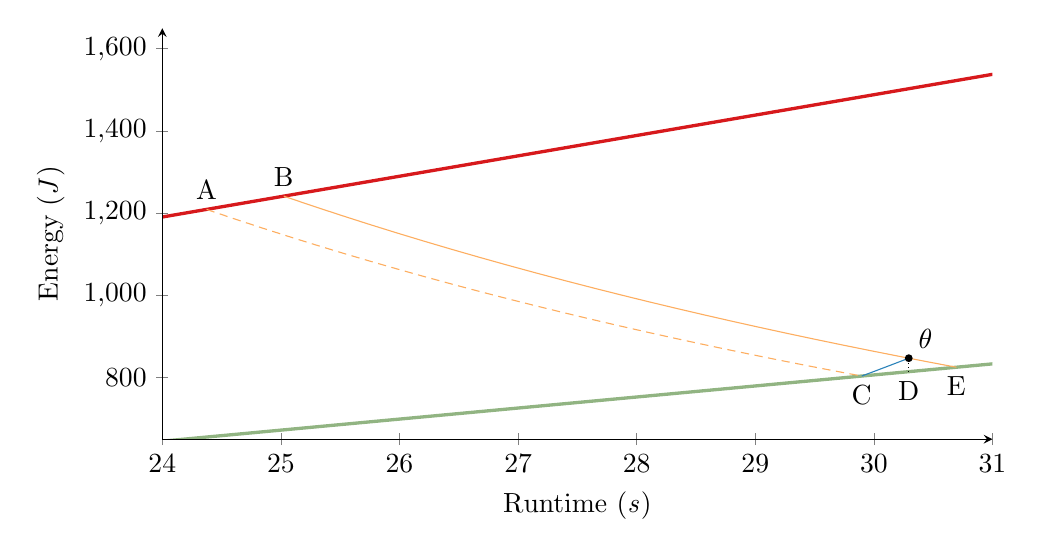
\begin{tikzpicture}
  \providecommand{\plotwidth}{\linewidth}
  \begin{axis}[
    axis on top,
    axis x line=bottom,
    axis y line=left,
    xlabel={Runtime (\emph{s})},
    ylabel={Energy (\emph{J})},    
    xmin=24, xmax=31,
    ymin=650, ymax=1650,
    width=\plotwidth,
    height=6.8cm,
    legend columns=3,
    legend to name=minimd:legend,
    legend style={/tikz/every even column/.append style={column sep=0.2cm}} % space out columns a bit
    ]

    %% Model Parameters %%
    \pgfmathsetmacro{\baselinepower}{26.876067}
    \pgfmathsetmacro{\rooflinepower}{49.60612}
    \pgfmathsetmacro{\codepower}{27.95947000000066} 
    \pgfmathsetmacro{\codetime}{30.293834}
    \pgfmathsetmacro{\codeenergy}{846.999542908}
    \pgfmathsetmacro{\energyexp}{1.0}
    \pgfmathsetmacro{\timeexp}{2.0}

    % Sadly, pgfplots sucks too much to calculate cube roots
    % These values are calculated with a ruby script in tools
    \pgfmathsetmacro{\blnodex}{29.897382525363728}
    \pgfmathsetmacro{\brnodex}{30.69554258273286}
    \pgfmathsetmacro{\trnodex}{25.0237350439618}
    \pgfmathsetmacro{\tlnodex}{24.373056016397907}

    %% Intermezzo Values %%
    \pgfmathsetmacro{\brnodey}{\brnodex * \baselinepower}
    \pgfmathsetmacro{\blnodey}{\blnodex * \baselinepower}
    \pgfmathsetmacro{\tlnodey}{\tlnodex * \rooflinepower}
    \pgfmathsetmacro{\trnodey}{\trnodex * \rooflinepower}
    \pgfmathsetmacro{\codeenergy}{\codepower * \codetime}
    \pgfmathsetmacro{\baselineenergy}{\baselinepower * \codetime}

    % arguments: code power, code time, x - todo, apparently not supposed to do pgfmathparse
    \pgfmathdeclarefunction{metricbound}{3}{%
      \pgfmathparse{((#1 * #2^3) / #3^2)}%
    }
    \pgfmathdeclarefunction{definitionbound}{3}{%
      \pgfmathparse{((#1 / #2^3) * #3^4)}%
    }

   % BETA ROOFLINE BOUND 
    \addplot[color=printred, very thick, domain=\pgfkeysvalueof{/pgfplots/xmin}:\pgfkeysvalueof{/pgfplots/xmax}] {\rooflinepower * x};
    \addlegendentry{$P_{max}$ Energy Bound}

    % ALPHA BASELINE BOUND 
    \addplot[color=printgreen, very thick, domain=\pgfkeysvalueof{/pgfplots/xmin}:\pgfkeysvalueof{/pgfplots/xmax}] {\baselinepower * x};
    \addlegendentry{$P_{min}$ Energy Bound} 

    \addplot[color=printorange, domain=\trnodex:\brnodex] { metricbound(\codepower, \codetime, x)};
    \addlegendentry{Optimisation Bound}

    \addplot[color=printblue, domain=\blnodex:\codetime] { definitionbound(\codepower, \codetime, x)};
    \addlegendentry{Contribution Bound}

    \addplot[color=printorange, densely dashed, domain=\tlnodex:\blnodex] {metricbound(\baselinepower, \blnodex, x)};
    \addlegendentry{Optimisation Limit}

    % Constant Time (Vertical) dotted line
    \draw[densely dotted] ({axis cs:\codetime,\baselineenergy}) -- ({axis cs:\codetime,\codeenergy});

    \node[circle,fill,inner sep=1pt] at (axis cs:\codetime,\codeenergy) {};
    \node[above right] at (axis cs:\codetime,\codeenergy) {$\theta$};
    
    \node [above] at ({axis cs:\tlnodex, \tlnodey}) {A};
    \node [above] at ({axis cs:\trnodex, \trnodey}) {B};
    \node [below] at ({axis cs:\blnodex, \blnodey}) {C};
    \node [below] at ({axis cs:\codetime,\baselineenergy}) {D};
    \node [below] at ({axis cs:\brnodex, \brnodey}) {E};
 \end{axis}
\end{tikzpicture}
%
    \caption{MiniMD}%
    \label{fig:minimd_pose}
  \end{subfigure}%
  \begin{subfigure}[t]{.5\linewidth}%
    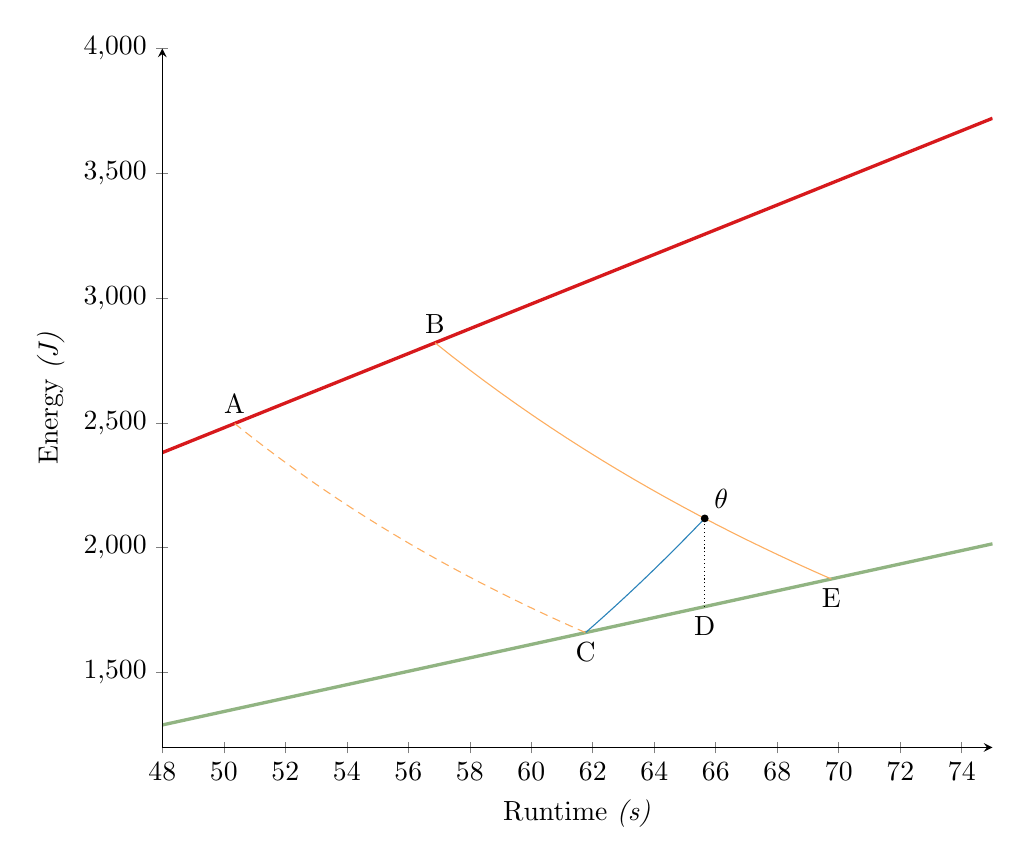
\begin{tikzpicture}
  \providecommand{\plotwidth}{\linewidth}
  \begin{axis}[
    axis on top,
    axis x line=bottom,
    axis y line=left,
  	xlabel={Runtime \emph{(s)}},
    ylabel={Energy \emph{(J)}},    
    xmin=48, xmax=75,
    ymin=1200, ymax=4000,
    width=\plotwidth,
    legend to name=lavamd:legend
    ]


    %% Model Parameters %%
    \pgfmathsetmacro{\baselinepower}{26.876067}
    \pgfmathsetmacro{\rooflinepower}{49.60612}
    \pgfmathsetmacro{\codepower}{32.25937199992712} 
    \pgfmathsetmacro{\codetime}{65.640072}
    \pgfmathsetmacro{\codeenergy}{2117.50750075}
    \pgfmathsetmacro{\energyexp}{1.0}
    \pgfmathsetmacro{\timeexp}{2.0}

    % Sadly, pgfplots sucks too much to calculate cube roots
    % These values are calculated with a ruby script in tools
    \pgfmathsetmacro{\blnodex}{61.76450770785698}
    \pgfmathsetmacro{\brnodex}{69.75881800183261}
    \pgfmathsetmacro{\trnodex}{56.869044551106185}
    \pgfmathsetmacro{\tlnodex}{50.35189300975517}
   
    %% Intermezzo Values %%
    \pgfmathsetmacro{\brnodey}{\brnodex * \baselinepower}
    \pgfmathsetmacro{\blnodey}{\blnodex * \baselinepower}
    \pgfmathsetmacro{\tlnodey}{\tlnodex * \rooflinepower}
    \pgfmathsetmacro{\trnodey}{\trnodex * \rooflinepower}
    \pgfmathsetmacro{\codeenergy}{\codepower * \codetime}
    \pgfmathsetmacro{\baselineenergy}{\baselinepower * \codetime}

    % arguments: code power, code time, x - todo, apparently not supposed to do pgfmathparse
    \pgfmathdeclarefunction{metricbound}{3}{%
      \pgfmathparse{((#1 * #2^3) / #3^2)}%
    }
    \pgfmathdeclarefunction{definitionbound}{3}{%
      \pgfmathparse{((#1 / #2^3) * #3^4)}%
    }


   % BETA ROOFLINE BOUND 
    \addplot[color=printred, very thick, domain=\pgfkeysvalueof{/pgfplots/xmin}:\pgfkeysvalueof{/pgfplots/xmax}] {\rooflinepower * x};
    \addlegendentry{$P_{max}$ Energy Bound}

    % ALPHA BASELINE BOUND 
    \addplot[color=printgreen, very thick, domain=\pgfkeysvalueof{/pgfplots/xmin}:\pgfkeysvalueof{/pgfplots/xmax}] {\baselinepower * x};
    \addlegendentry{$P_{min}$ Energy Bound} 

    \addplot[color=printorange, domain=\trnodex:\brnodex] { metricbound(\codepower, \codetime, x)};
    \addlegendentry{Optimisation Bound}

    \addplot[color=printblue, domain=\blnodex:\codetime] { definitionbound(\codepower, \codetime, x)};
    \addlegendentry{Contribution Bound}

    \addplot[color=printorange, densely dashed, domain=\tlnodex:\blnodex] {metricbound(\baselinepower, \blnodex, x)};
    \addlegendentry{Optimisation Limit}

    % Constant Time (Vertical) dotted line
    \draw[densely dotted] ({axis cs:\codetime,\baselineenergy}) -- ({axis cs:\codetime,\codeenergy});

    \node[circle,fill,inner sep=1pt] at (axis cs:\codetime,\codeenergy) {};
    \node[above right] at (axis cs:\codetime,\codeenergy) {$\theta$};
    
    \node [above] at ({axis cs:\tlnodex, \tlnodey}) {A};
    \node [above] at ({axis cs:\trnodex, \trnodey}) {B};
    \node [below] at ({axis cs:\blnodex, \blnodey}) {C};
    \node [below] at ({axis cs:\codetime,\baselineenergy}) {D};
    \node [below] at ({axis cs:\brnodex, \brnodey}) {E};
 \end{axis}
\end{tikzpicture}
%
    \caption{LavaMD}%
    \label{fig:lavamd_pose}
  \end{subfigure}%
  \begin{center}%
    \ref{minimd:legend}%
  \end{center}%
  \caption{$E^1t^2$ POSE comparison}%
  \label{fig:comparison}%
\end{figure*}


\subsection{POSE Models for Frequency Scaling}
\noindent
The relationship between P-state and energy consumption is non-linear and workload dependent.
Operating in low power states can increase runtime, offsetting any energy savings from reduced power draw~\cite{le:2010aa}.
Application-aware DVFS can save energy by selecting the optimal P-state schedule for a given code~\cite{choi:2004aa}.
This implies that code changes may effect the optimal P-state assignment. 
We now use POSE to reason about this class of optimisation.

The performance of MiniMD and LavaMD was measured for each P-state supported by our system.
\autoref{fig:pstates} shows that the energy consumption of both codes can be reduced at the cost of increased runtime.
Despite this, the lowest $E^1t^2$ value for both codes occurs at 3.2 GHz, meaning race-to-halt is the optimal strategy in terms of this metric. 

While useful, this simple analysis fails to account for potential co-opti\-misa\-tion of activity factor and P-state.
It is possible that different optimisations may be required to achieve optimal performance in different P-states.
The flexibility of POSE allows us to model this scenario by considering optimisations which can impact P-state as well as activity factor.
\autoref{eq:pbfreq} gives the feasible performance envelope corresponding to this class of optimisation.

\begin{align}
  \label{eq:pbfreq}
  \begin{split}
    P_{min} &= (1.6\text{ GHz}, \alpha, 4) = 13.51W, \\
    P_{max} &= (3.2\text{ GHz}, \beta, 4) = 49.61W
  \end{split}
\end{align}

\begin{figure*}[t]%
  \scriptsize
\begin{subfigure}[t]{.5\linewidth}%
\@ifundefined{pstateminimdtable}{%
  \pgfplotstableread[col sep=comma]{plot/minimd-pstates/data/pstate_power_4_cores.csv}\pstateminimdtable
}{}

\begin{tikzpicture}
  \begin{axis}[
    width=0.95\linewidth,
    axis on top,
    axis x line=bottom,
    axis y line=left,
  	xlabel={Runtime \emph{(s)}},
    ylabel={Energy \emph{(J)}},    
    xmin=0, xmax=60,
    ymin=0, ymax=1500,
    legend columns=2,
    legend to name=minimd-pstate:legend,
    legend style={/tikz/every even column/.append style={column sep=0.2cm}} % space out columns a bit
    ]

    %% Model Parameters %%
    \pgfplotstablegetelem{0}{Runtime}\of{\pstateminimdtable}
    \pgfmathsetmacro{\codetime}{\pgfplotsretval} 
    \pgfplotstablegetelem{0}{Energy}\of{\pstateminimdtable}
    \pgfmathsetmacro{\codeenergy}{\pgfplotsretval} 
    \pgfmathsetmacro{\baselinepower}{13.510238}

    %% Intermezzo Values %%
    \pgfmathsetmacro{\codepower}{\codeenergy / \codetime}

    % arguments: code power, code time, x, n 
    \pgfmathdeclarefunction{metricbound}{4}{%
      \pgfmathparse{((#1 * #2^(#4 + 1)) / #3^#4)}%
    }
    \pgfmathdeclarefunction{definitionbound}{4}{%
      \pgfmathparse{((#1 / #2^(#4 + 1)) * #3^(#4 + 2))}%
    }

    % ALPHA BASELINE BOUND 
    \addplot[color=printgreen, very thick, name path=basebound, domain=\pgfkeysvalueof{/pgfplots/xmin}:\pgfkeysvalueof{/pgfplots/xmax}] {\baselinepower * x};
    \addlegendentry{$P_{min}$ Energy Bound} 


    %% 3.2 GHz start point
    \pgfmathsetmacro{\blnodex}{23.77199310523716}
    \pgfmathsetmacro{\brnodex}{38.6049404590049}
    \addplot[name path=edpdef, draw=none, domain=\blnodex:\codetime+1, forget plot] {definitionbound(\codepower, \codetime, x, 2)};
    \addplot[name path=edpopt, draw=none, domain=\codetime-1:\brnodex, forget plot] {metricbound(\codepower, \codetime, x, 2)};

    \path[name path=edpspace,
      intersection segments={
        of=edpdef and edpopt,
        sequence=A0 -- B1,
      }
      ]; 
    \addplot[blue!20] fill between[of=edpspace and basebound]; 
    \addlegendentry{3.2 GHz POSE}

    %% PState progression
    \addplot[mark=x, black] table[x=Runtime,y=Energy, trim cells=true] {\pstateminimdtable}
      node[pos=0.0, pin=left:3.2 GHz]{}
      node[pos=1.0, pin=95:1.6 GHz]{}
      node[pos=0.5745, pin={[pin distance=0.15cm] above:2.2 GHz}]{}
    ;
    \addlegendentry{P-state Progression}

    %%
    \pgfmathsetmacro{\codetime}{31.160996}
    \pgfmathsetmacro{\codepower}{26.555410070974624}
    \pgfmathsetmacro{\blnodex}{24.876044579784466}
    \addplot[name path=edpdef, gray, densely dashed, domain=\blnodex:\codetime, forget plot] {definitionbound(\codepower, \codetime, x, 2)};

    %%
    \pgfmathsetmacro{\codetime}{32.221644}
    \pgfmathsetmacro{\codepower}{25.19066851461707}
    \pgfmathsetmacro{\blnodex}{26.17914532437151}
    \addplot[name path=edpdef, gray, densely dashed, domain=\blnodex:\codetime, forget plot] {definitionbound(\codepower, \codetime, x, 2)};

    %%
    \pgfmathsetmacro{\codetime}{33.189564}
    \pgfmathsetmacro{\codepower}{24.052689996168674}
    \pgfmathsetmacro{\blnodex}{27.384280155637242}
    \addplot[name path=edpdef, gray, densely dashed, domain=\blnodex:\codetime, forget plot] {definitionbound(\codepower, \codetime, x, 2)};

    %%
    \pgfmathsetmacro{\codetime}{35.548669}
    \pgfmathsetmacro{\codepower}{21.708309894809283}
    \pgfmathsetmacro{\blnodex}{30.35072062021389}
    \addplot[name path=edpdef, gray, densely dashed, domain=\blnodex:\codetime, forget plot] {definitionbound(\codepower, \codetime, x, 2)};

    %%
    \pgfmathsetmacro{\codetime}{36.852917}
    \pgfmathsetmacro{\codepower}{20.791885293639034}
    \pgfmathsetmacro{\blnodex}{31.919904165043228}
    \addplot[name path=edpdef, gray, densely dashed, domain=\blnodex:\codetime, forget plot] {definitionbound(\codepower, \codetime, x, 2)};

    %%
    \pgfmathsetmacro{\codetime}{38.225746}
    \pgfmathsetmacro{\codepower}{19.926273930664426}
    \pgfmathsetmacro{\blnodex}{33.58161699951163}
    \addplot[name path=edpdef, gray, densely dashed, domain=\blnodex:\codetime, forget plot] {definitionbound(\codepower, \codetime, x, 2)};

    %%
    \pgfmathsetmacro{\codetime}{39.720356}
    \pgfmathsetmacro{\codepower}{19.032817706870503}
    \pgfmathsetmacro{\blnodex}{35.432334683311204}
    \addplot[name path=edpdef, gray, densely dashed, domain=\blnodex:\codetime, forget plot] {definitionbound(\codepower, \codetime, x, 2)};

    %%
    \pgfmathsetmacro{\codetime}{41.430395}
    \pgfmathsetmacro{\codepower}{18.26008617586195}
    \pgfmathsetmacro{\blnodex}{37.47190734697387}
    \addplot[name path=edpdef, gray, densely dashed, domain=\blnodex:\codetime, forget plot] {definitionbound(\codepower, \codetime, x, 2)};

    %% 2.2GHz
    \pgfmathsetmacro{\codetime}{43.161913}
    \pgfmathsetmacro{\codepower}{17.552650110758528}
    \pgfmathsetmacro{\blnodex}{39.55555231782452}
    \addplot[name path=edpdef, red, densely dashed, domain=\blnodex:\codetime] {definitionbound(\codepower, \codetime, x, 2)};
    \addlegendentry{Optimisation Cutoff}

    %%
    \pgfmathsetmacro{\codetime}{45.85507}
    \pgfmathsetmacro{\codepower}{16.61222678321067}
    \pgfmathsetmacro{\blnodex}{42.802165661611}
    \addplot[name path=edpdef, gray, densely dashed, domain=\blnodex:\codetime, forget plot] {definitionbound(\codepower, \codetime, x, 2)};

    %%
    \pgfmathsetmacro{\codetime}{49.7305}
    \pgfmathsetmacro{\codepower}{15.67846259337831}
    \pgfmathsetmacro{\blnodex}{47.323406701270244}
    \addplot[name path=edpdef, gray, densely dashed, domain=\blnodex:\codetime, forget plot] {definitionbound(\codepower, \codetime, x, 2)};

    %%
    \pgfmathsetmacro{\codetime}{52.358683}
    \pgfmathsetmacro{\codepower}{15.137478343372388}
    \pgfmathsetmacro{\blnodex}{50.41098720057872}
    \addplot[name path=edpdef, gray, densely dashed, domain=\blnodex:\codetime, forget plot] {definitionbound(\codepower, \codetime, x, 2)};

    %%
    \pgfmathsetmacro{\codetime}{55.340763}
    \pgfmathsetmacro{\codepower}{14.650088958838532}
    \pgfmathsetmacro{\blnodex}{53.866578212248804}
    \addplot[name path=edpdef, gray, densely dashed, domain=\blnodex:\codetime, forget plot] {definitionbound(\codepower, \codetime, x, 2)};

    %%
    \pgfmathsetmacro{\codetime}{58.637567}
    \pgfmathsetmacro{\codepower}{14.09304050763225}
    \pgfmathsetmacro{\blnodex}{57.81786383949271}
    \addplot[name path=edpdef, gray, densely dashed, domain=\blnodex:\codetime, forget plot] {definitionbound(\codepower, \codetime, x, 2)};


 \end{axis}
\end{tikzpicture}
%
\caption{MiniMD}%
\label{fig:minimd-pstates}%
\end{subfigure}%
\begin{subfigure}[t]{.5\linewidth}%
\@ifundefined{pstatelavamdtable}{%
  \pgfplotstableread[col sep=comma]{plot/lavamd-pstates/data/pstate_power_4_cores.csv}\pstatelavamdtable
}{}

\begin{tikzpicture}
  \begin{axis}[
    width=0.95\linewidth,
    axis on top,
    axis x line=bottom,
    axis y line=left,
  	xlabel={Runtime \emph{(s)}},
    ylabel={Energy \emph{(J)}},    
    xmin=0, xmax=140,
    ymin=0, ymax=3800,
    legend columns=2,
    legend to name=lavamd-pstate:legend,
    legend style={/tikz/every even column/.append style={column sep=0.2cm}} % space out columns a bit
    ]

    %% Model Parameters %%
    \pgfplotstablegetelem{0}{Runtime}\of{\pstatelavamdtable}
    \pgfmathsetmacro{\codetime}{\pgfplotsretval} 
    \pgfplotstablegetelem{0}{Energy}\of{\pstatelavamdtable}
    \pgfmathsetmacro{\codeenergy}{\pgfplotsretval} 
    \pgfmathsetmacro{\baselinepower}{13.510238}

    %% Intermezzo Values %%
    \pgfmathsetmacro{\codepower}{\codeenergy / \codetime}

    % arguments: code power, code time, x, n 
    \pgfmathdeclarefunction{metricbound}{4}{%
      \pgfmathparse{((#1 * #2^(#4 + 1)) / #3^#4)}%
    }
    \pgfmathdeclarefunction{definitionbound}{4}{%
      \pgfmathparse{((#1 / #2^(#4 + 1)) * #3^(#4 + 2))}%
    }

    % ALPHA BASELINE BOUND 
    \addplot[color=green, name path=basebound, domain=\pgfkeysvalueof{/pgfplots/xmin}:\pgfkeysvalueof{/pgfplots/xmax}] {\baselinepower * x};
    \addlegendentry{$P_{min}$ Energy Bound} 


    %% 3.2 GHz start point
    \pgfmathsetmacro{\brnodex}{87.73374843784023}
    \pgfmathsetmacro{\blnodex}{49.11016716922632}
    \addplot[name path=edpdef, draw=none, domain=\blnodex:\codetime+1, forget plot] {definitionbound(\codepower, \codetime, x, 2)};
    \addplot[name path=edpopt, draw=none, domain=\codetime-1:\brnodex, forget plot] {metricbound(\codepower, \codetime, x, 2)};

    \path[name path=edpspace,
      intersection segments={
        of=edpdef and edpopt,
        sequence=A0 -- B1,
      }
      ]; 
    \addplot[blue!20] fill between[of=edpspace and basebound]; 
    \addlegendentry{3.2 GHz POSE}

    %% PState progression
    \addplot[mark=x, black] table[x=Runtime,y=Energy, trim cells=true] {\pstatelavamdtable}
      node[pos=0.0, pin=left:3.2 GHz]{}
      node[pos=1.0, pin=95:1.6 GHz]{}
      node[pos=0.636, pin={[pin distance=0.15cm] above:2.1 GHz}]{}
    ;
    \addlegendentry{P-State Progression}


    %%
    \pgfmathsetmacro{\codetime}{67.788671}
    \pgfmathsetmacro{\codepower}{30.534496154969613}
    \pgfmathsetmacro{\blnodex}{51.65525781584337}
    \addplot[name path=edpdef, gray, densely dashed, domain=\blnodex:\codetime, forget plot] {definitionbound(\codepower, \codetime, x, 2)};

    %%
    \pgfmathsetmacro{\codetime}{69.909725}
    \pgfmathsetmacro{\codepower}{28.972621505806238}
    \pgfmathsetmacro{\blnodex}{54.21207070239038}
    \addplot[name path=edpdef, gray, densely dashed, domain=\blnodex:\codetime, forget plot] {definitionbound(\codepower, \codetime, x, 2)};

    %%
    \pgfmathsetmacro{\codetime}{72.820343}
    \pgfmathsetmacro{\codepower}{27.23156518227331}
    \pgfmathsetmacro{\blnodex}{57.647815146592066}
    \addplot[name path=edpdef, gray, densely dashed, domain=\blnodex:\codetime, forget plot] {definitionbound(\codepower, \codetime, x, 2)};

    %%
    \pgfmathsetmacro{\codetime}{78.83738}
    \pgfmathsetmacro{\codepower}{24.363863791516156}
    \pgfmathsetmacro{\blnodex}{64.76958711476986}
    \addplot[name path=edpdef, gray, densely dashed, domain=\blnodex:\codetime, forget plot] {definitionbound(\codepower, \codetime, x, 2)};

    %%
    \pgfmathsetmacro{\codetime}{80.443575}
    \pgfmathsetmacro{\codepower}{23.569310575766927}
    \pgfmathsetmacro{\blnodex}{66.82363092159444}
    \addplot[name path=edpdef, gray, densely dashed, domain=\blnodex:\codetime, forget plot] {definitionbound(\codepower, \codetime, x, 2)};

    %%
    \pgfmathsetmacro{\codetime}{83.583275}
    \pgfmathsetmacro{\codepower}{22.42571518045925}
    \pgfmathsetmacro{\blnodex}{70.59245458487962}
    \addplot[name path=edpdef, gray, densely dashed, domain=\blnodex:\codetime, forget plot] {definitionbound(\codepower, \codetime, x, 2)};

    %%
    \pgfmathsetmacro{\codetime}{87.25231}
    \pgfmathsetmacro{\codepower}{21.415643975500476}
    \pgfmathsetmacro{\blnodex}{74.83203474018039}
    \addplot[name path=edpdef, gray, densely dashed, domain=\blnodex:\codetime, forget plot] {definitionbound(\codepower, \codetime, x, 2)};

    %%
    \pgfmathsetmacro{\codetime}{90.581583}
    \pgfmathsetmacro{\codepower}{20.54295973167084}
    \pgfmathsetmacro{\blnodex}{78.77224707386881}
    \addplot[name path=edpdef, gray, densely dashed, domain=\blnodex:\codetime, forget plot] {definitionbound(\codepower, \codetime, x, 2)};

    %%
    \pgfmathsetmacro{\codetime}{95.357508}
    \pgfmathsetmacro{\codepower}{19.637888418812288}
    \pgfmathsetmacro{\blnodex}{84.1803958382032}
    \addplot[name path=edpdef, gray, densely dashed, domain=\blnodex:\codetime, forget plot] {definitionbound(\codepower, \codetime, x, 2)};

    %%
    \pgfmathsetmacro{\codetime}{99.502899}
    \pgfmathsetmacro{\codepower}{18.820670933416725}
    \pgfmathsetmacro{\blnodex}{89.0932975465577}
    \addplot[name path=edpdef, red, densely dashed, domain=\blnodex:\codetime] {definitionbound(\codepower, \codetime, x, 2)};
    \addlegendentry{Optimization Boundary}
    %%
    \pgfmathsetmacro{\codetime}{109.970804}
    \pgfmathsetmacro{\codepower}{17.334285425429826}
    \pgfmathsetmacro{\blnodex}{101.20370662532102}
    \addplot[name path=edpdef, gray, densely dashed, domain=\blnodex:\codetime, forget plot] {definitionbound(\codepower, \codetime, x, 2)};

    %%
    \pgfmathsetmacro{\codetime}{115.469869}
    \pgfmathsetmacro{\codepower}{16.703561489274747}
    \pgfmathsetmacro{\blnodex}{107.58539357794623}
    \addplot[name path=edpdef, gray, densely dashed, domain=\blnodex:\codetime, forget plot] {definitionbound(\codepower, \codetime, x, 2)};

    %%
    \pgfmathsetmacro{\codetime}{123.182269}
    \pgfmathsetmacro{\codepower}{16.060352379123653}
    \pgfmathsetmacro{\blnodex}{116.28334319474206}
    \addplot[name path=edpdef, gray, densely dashed, domain=\blnodex:\codetime, forget plot] {definitionbound(\codepower, \codetime, x, 2)};

    %%
    \pgfmathsetmacro{\codetime}{130.924339}
    \pgfmathsetmacro{\codepower}{15.486518591474423}
    \pgfmathsetmacro{\blnodex}{125.09985043035239}
    \addplot[name path=edpdef, gray, densely dashed, domain=\blnodex:\codetime, forget plot] {definitionbound(\codepower, \codetime, x, 2)};
  \end{axis}
\end{tikzpicture}
%
\caption{LavaMD}%
\label{fig:lavamd-pstates}%
\end{subfigure}%
\begin{center}%
\ref{minimd-pstate:legend}%
\end{center}%
\caption{$E^1t^2$ POSE for P-state Optimisation}%
\label{fig:pstates}%
\end{figure*}%

We choose the 3.2 GHz run as our initial `unoptimised' baseline because this is the P-state our system defaults to when running MiniMD or LavaMD.
If the POSE models for two P-states do not overlap then switching to the higher performance P-state outperforms any possible power optimisation at the weaker state.
This state can then be excluded from any search for power optimisations.

For MiniMD, \autoref{fig:minimd-pstates} shows that the first POSE model which does not overlap with the one built for our baseline occurs at 2.2 GHz.
This means no power optimisations exists at P-states 2.2 GHz and below which can match the $E^1t^2$ performance of our unoptimised baseline.
Conversely, such an optimisation may exist at frequencies between 3.2 GHz and 2.2 GHz as shown by the overlapping of the respective POSE models.
For LavaMD this optimisation threshold is slightly lower at 2.1 GHz, lending support to the claim that of these two codes LavaMD is more amenable to power optimisation.

Dynamic Concurrency Throttling has also been proposed as a means to reduce energy consumption~\cite{maury:2006aa}.
It would be trivial to use POSE to model optimisations which influence core count.
The only difference between this and our DVFS investigation would be slightly different parameterisation of the feasible performance envelope ($C_{min}=1$).

  \section{Conclusion}
\label{sec:conclusion}
\noindent
This paper presents POSE, a mathematical and visual model which captures the energy/runtime optimisation trade-off space of a code.
POSE is a robust analytical model which provides developers with quantitative and actionable insights.
The main use case for POSE is helping to determine whether power or runtime optimisation is the best approach for improving the efficiency of a code.

POSE works by partitioning the energy/runtime plane into areas corresponding to runtime and power optimised versions of an initial code with respect to a cost metric.
We provide derivations of POSE's boundaries for the Energy Delay Squared family of metrics.
We also demonstrate how to apply POSE in practice by modelling the CPU power consumption of a number of codes taken from the Rodinia and Mantevo benchmark suites.  

The results in this paper illustrate that runtime optimisation is the preferred approach to reducing the energy consumption of MiniMD and to a lesser extent LavaMD.
Our investigation into frequency scaling also highlights the ability of POSE to rule out dominated configurations and hence reduce the optimisation search space.
We believe that both results are of interest to performance engineers and serve to demonstrate the practical utility of POSE.

POSE is under consideration for inclusion into a state of the art application analytics for HPC clusters and applications \textit{[paragraph redacted to preserve anonymity]}.

\subsection*{Future Work}
\noindent
Future work will further validate POSE by applying it to a broader selection of scientific codes running on a range of machines.
The quantitative nature of our technique makes it particularly well suited to comparison studies.
As such, we are particularly keen to investigate the power optimisation opportunities presented by different architectures.

Our ultimate aim is to demonstrate how POSE may be used to identify specific optimisations.
This will involve developing feasible performance envelopes for individual subsystems including memory, file systems and processors. 
We also intend to profile specific classes of code and establish $P_{min}$ baselines for each.
Doing so would allow POSE to highlight optimisation opportunities at a per-kernel, per-subsystem level and hence facilitate targeted optimisation.

  \bibliographystyle{plain}
  \bibliography{bib/all} 
\end{document}
